
\section{Summary of papers}
\label{sec:summary}
In this final introductory section we summarize the papers that make
up this thesis, and we also give some final concluding remarks
and future directions. 

\subsection{Paper 1: High-resolution data assimilation of cardiac mechanics
  applied to a dyssynchronous ventricle}



\begin{figure}[htbp]
  \centering
    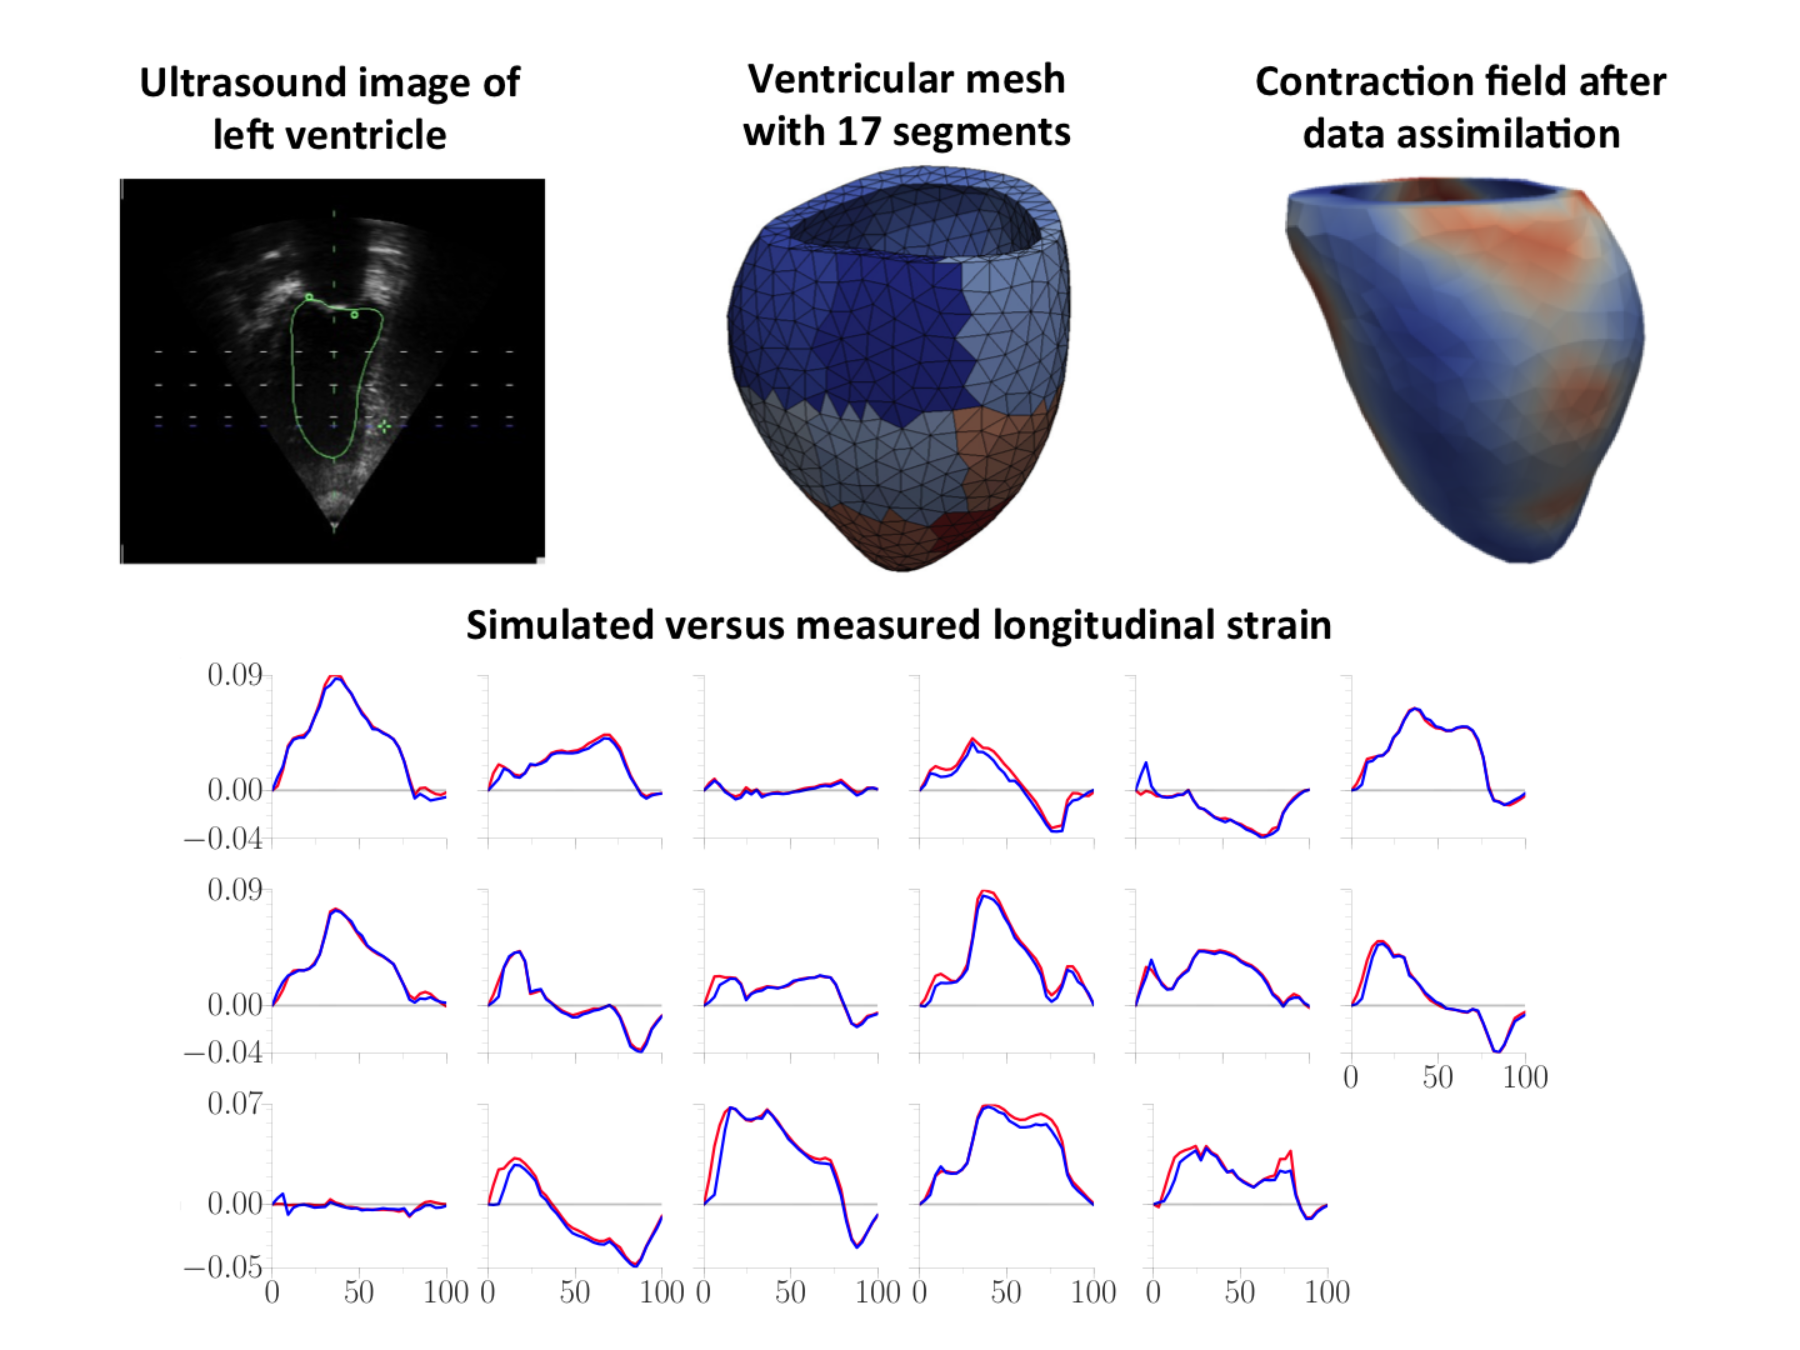
\includegraphics[width=0.8\textwidth]{chapters/introduction/figures/paper1}
\caption{Summary figure for paper 1}
\label{fig:paper1}
\end{figure}


In this paper we develop and test a pipeline for constructing a
patient-specific mechanical simulation of a patient's heart, based on
clinical measurements and adjoint-based data assimilation
techniques.

As a model case we consider one patient, diagnosed with
left bundle branch block and selected for cardiac resynchronization
therapy (CRT). Prior to the CRT implantation the patient had 4D
echocardiography taken for which the LV geometry, LV volumes and LV
regional strains throughout the cardiac cycle are measured. During
implantation of the CRT device the LV pressure were also measured
invasively. The LV pressure measurements were used as boundary condition at the
endocardium, while the LV volume and LV regional strain were incorporated
into a cost functional that we wanted to minimize.


The pipeline is divided into two phases, a passive phase where we
estimate the linear isotropic parameters $a$ in
\eqref{eq:holzapel_trans} as a global material parameter using the
measurement points belonging atrial systole, and an active phase where we estimate
a spatially varying contraction parameter ($\gamma$ in
\eqref{eq:intro_active_strain_Fa_gjerald}) at each measurement point
with active contraction. During the passive phase we only fit the
volumes, while during the active phase a total of 51 strain measurements in the radial,
longitudinal and circumferential direction in each AHA segment (Figure
\ref{fig:echopac_output}) were used additionally in the optimization. 

The results show an excellent fit with measured strain an volume, with
a average relative error in the volume and strain of less than 0.4 \% and 3 \%
respectively using a contraction parameter with one degree of freedom
for each vertex in the geometry (2661 parameters in total). Parameters
at lower spatial resolution are also tested to show the necessity of
high spatial resolution to fit the measured strain data.
A synthetic test is also performed in order to show that the method
is able to recapitulate the generated data, also with noise added to
the data. Moreover, a sensitivity analysis to different parameters are
presented in the appendix.


\subsection{Paper 2: Estimating cardiac contraction through high resolution
  data assimilation of a personalized mechanical model}


\begin{figure}[htbp]
  \centering
    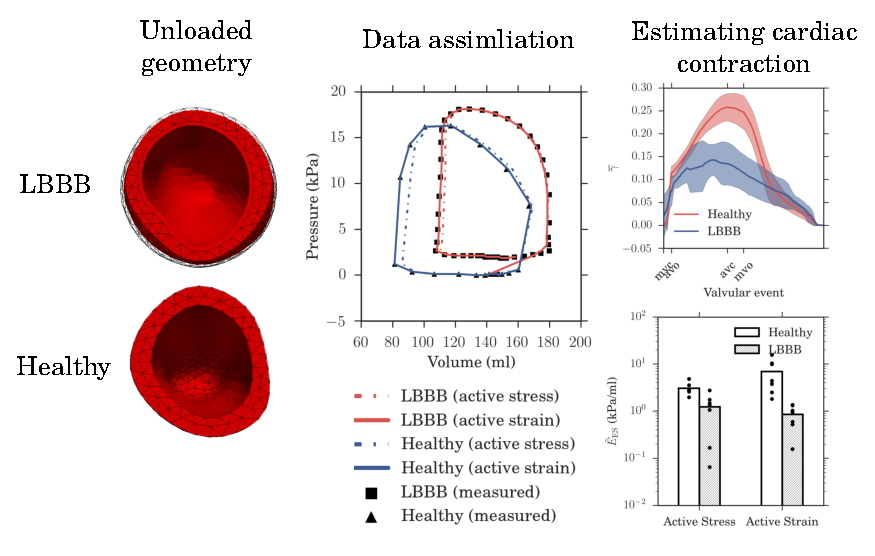
\includegraphics[width=0.8\textwidth]{chapters/introduction/figures/paper2}
\caption{Summary figure for paper 2}
\label{fig:paper2}
\end{figure}

In this paper we apply the method developed in the previous paper to a
cohort of patients and estimate indices of cardiac contractility. More
specifically, a group of seven patients diagnosed with left bundle branch block and
selected for cardiac resynchronization therapy (CRT), and a group of
seven healthy control subjects were included in the study.

The pipeline is similar to the one outlined in paper 1, with the
exception that we also estimate the unloaded, stress-free
configuration using the method outlined in Section
\ref{sec:intro_coupled_material}. 

The optimized active strain parameter in
\eqref{eq:intro_active_strain_Fa_gjerald} as well as the optimized
active stress parameter in \eqref{eq:intro_active_stress} are averaged
over the ventricle and compared between the two groups. The healthy
group showed a significant increase in both of these
parameters. Furthermore, an estimation of the end-systolic elastance by
perturbation of the model at the end-systolic state, while fixing
the remaining quantities, was also conducted. This estimate of end-systolic
elastance were also significantly higher in the healthy control
group. 


\subsection{Paper 3: Efficient estimation of personalized biventricular mechanical
  function employing gradient-based optimizatio}

\begin{figure}[htbp]
  \centering
    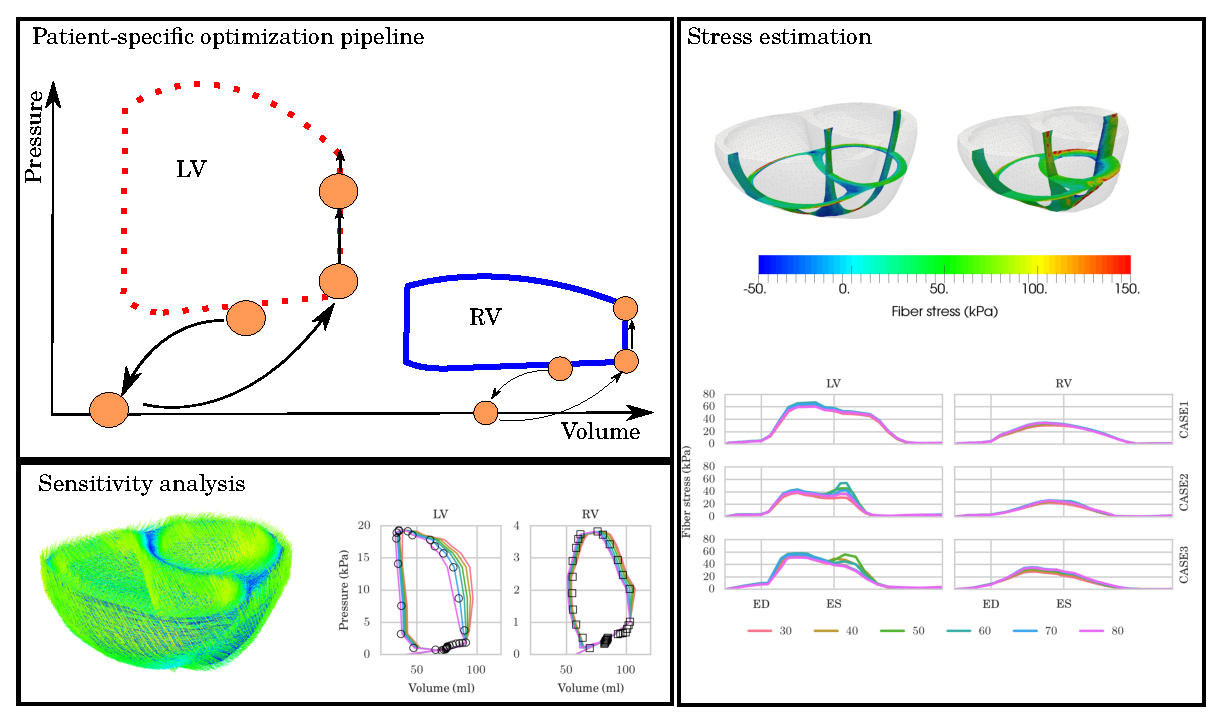
\includegraphics[width=0.75\textwidth]{chapters/introduction/figures/paper3}
\caption{Summary figure for paper 3}
\label{fig:paper3}
\end{figure}

In this paper we extend the work in the two previous paper to
bi-ventricular geometries, and use it to estimate patient-specific
myofiber stress and indices of contractility. Furthermore, we investigate
the sensitivity of these computed features the helical fiber angle and
the choice of active modeling framework.

In this work we estimate the linear isotopic material parameter in
\eqref{eq:holzapel_trans}, spatially resolved on the LV and RV, by
minimizing the error in end-diastolic LV and RV cavity volumes.
We use a simplified algorithm to estimate the unloaded geometry, since
the problem of estimating an unloaded BiV-geometry is not well-posed
because buckling of the RV free wall might occur. The amount of active
contraction is estimated during the active phase, by minimizing
simulated and measured volumes and circumferential strain. The active
control parameter, which are $\gamma$ in
\eqref{eq:intro_active_strain_Fa_gjerald}  and $T_a$ in
\eqref{eq:intro_active_stress} for the active strain and active stress
formulation respectively, are spatially resolved on the
LV free wall (LVFW), the RV free wall (RVFW) and the septum. With so
few control parameters, issues related to conflicting objectives, i.e
that is is not possible to minimize both the strain and volume, is
evident. However, with a low dimensional parameter space, questions
regarding identifiability and uniqueness of the estimated parameters
are easier to answer. In this study we also perform a validation of
the model, by comparing simulated and measured longitudinal strain
which is not used in the optimization. 

The results show low variability with respect to choice of fiber angle
and active modeling framework. Also, the fit of data depends upon the
choice of fiber angle, and a steeper fiber angle than previously
suggested, provides the best fit. The work here could potentially be
used to extract patient-specific maps of ventricular fiber stress and
contractility which could be useful in diagnostic of several heart
diseases related to heart failure. 




\subsection{Paper 4: Assessment of regional myocardial work from a
  patient-specific cardiac mechanics model}

\begin{figure}[htbp]
  \centering
    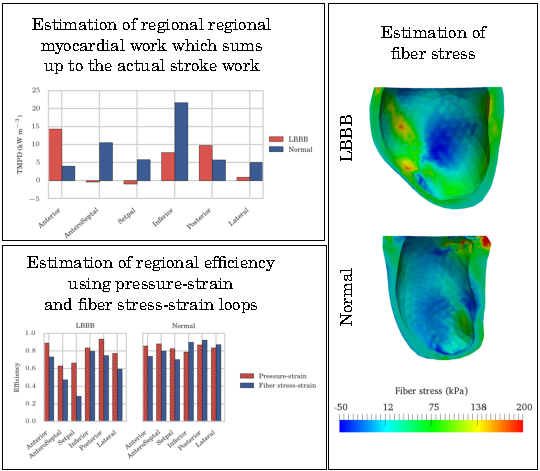
\includegraphics[width=0.7\textwidth]{chapters/introduction/figures/paper4}
\caption{Summary figure for paper 4}
\label{fig:paper3}
\end{figure}


In this paper we investigate if it is possible to assess regional
myocardial work using data assimilation and finite element modeling.
The amount of work performed by the left ventricle equals to the
amount to work needed to eject blood against the intraventricular
pressure. Effectively, a global measure of work is therefore the same
as the area of the pressure volume (PV) loop which is most commonly refered
to as stroke work.  However, stroke work is a global measure which
does not reflect whether some regions in the ventricle work harder than
others to compensate for regional dysfunction, in order to maintain the
stroke work needed to meet the body's demand. Therefore a regional
measure of work would be helpful in assessment of patients with
regional dysfunction, and preferable we would have a regional meausure
that summed up to the actual stroke work. The area of the
pressure-strain loops, where strain here refers to as regional
longitudinal strain, has been proposed as a meausure regional
myocardial work, and indices based on these work calculations have
shown to be a good predictor of response to cardiac resynchronization
therapy, a treatment given to patients with regional dysfunction.

To check the validity of these work calculations we estimate work
using well known laws from continuum mechanics in a personalized
cardiac mechanics model, similar to the models in the previous papers.
These work calculations are compared to estimates using the
pressure-strain loops approach, and to the ``gold-standard'' PV area.
Our estimates of global mechanical work are in good agreements with
estimated PV area, while the pressure-strain loops quantitatively
underestimates the total mechanical work. However, relative measures
of regional efficiency seems to be independent of how work is
computed, and yields the same results in terms of assesment of regional
dysfunction. Our finding therefore suggest that regional myocardial
work can be assessed using patient-specific finite element modeling,
while regional dysfunction in terms of indices of efficiency are
independent of how work is computed.

In this study we also perform a convergence analysis of the algorithm for
determining the unloaded, zero-pressure geometry as well as the
algorithm for joint estimation of material parameters and unloaded
geometry. 

\newpage
\section{Other contributions}
Along with the research articles presented in this thesis, other
types of contributions in terms of talks, posters and software has
been made during the writing of this thesis. These contributions are
listed below.

\subsection{Talks}
\begin{itemize}
  \item Henrik Finsberg, Gabriel Balaban, Joakim Sundnes, Hans
    Henrik Odland, Marie Rognes, and Samuel T. Wall. ``Patient
    Constrained Ventricular Stress Mapping'',
    Conference Presentation at MALT 2015,  Lugano, Switzerland (2015).
  \item Henrik Finsberg, Gabriel Balaban, Joakim Sundnes, Marie
    Rognes, and Samuel T. Wall. ``Personalization of a Cardiac
    Computational Model using Clinical Measurements'', Conference
    Presentation at 28th Nordic Seminar on Computational
    Mechanics. Vol. 28. Tallin, Estonia, (2015).
  \item Henrik Finsberg, Gabriel Balaban, Joakim Sundnes, Marie
    Rognes, and Samuel T. Wall. ``Optimization of a Spatially Varying
    Cardiac Contraction parameter using the Adjoint Method'',
    Conference Presentation at FEniCS 16, Oslo, Norway,(2016).
  \item Henrik Finsberg, Gabriel Balaban, Joakim Sundnes, Hans
    Henrik Odland, Marie Rognes, and Samuel T. Wall. ``Personalized
    Cardiac Mechanical Model using a High Resolution Contraction Field
    '',  Conference Presentation at VPH16 Translating VPH to the
    Clinic,  Amsterdam, Netherlands (2016).
  \item Henrik Finsberg, John Aalen,Camilla K.
    Larsen, Espen Remme, Joakim Sundnes, Otto A. Smiseth, and 
    Samuel T. Wall. ``Assessment of regional myocardial work via through
    adjoint-based data assimilation. '',  Conference Presentation at
    the International Conference on Computational Science and
    Enfineering, Oslo, Norway (2016).
\end{itemize}


\subsection{Posters}
\begin{itemize}
  \item Henrik Finsberg, Gabriel Balaban, Joakim Sundnes, Marie
    Rognes, and Samuel T. Wall. ``Patient Specific Modeling of Cardiac
    Mechanics using the Active Strain Formulation '',
    Geilo Winter School, Geilo, Norway, (2016).
  \item Henrik Finsberg, Ce Xi, J. Tan, L. Zhong, LC Lee, Joakim
    Sundnes, and Samuel T. Wall. ``Mechanical Analysis of Pulmonary
    Hypertension via Adjoint based Data Assimilation of a Finite
    Element Model '', Summer Biomechanics, Bioengineering, and
    Biotransport Conference, Tucson, AZ, (2017). 
  \end{itemize}


\subsection{Software}
\begin{itemize}
  \item Pulse-Adjoint, FEniCS-based cardiac mechanics solver and data
    assimilator, source: \url{https://bitbucket.org/finsberg/pulse_adjoint}
  \item Mesh-Toolbox, Toolbox for generating FEniCS meshes from 4D
    Echo,  source: \url{https://bitbucket.org/finsberg/mesh_generation}
\end{itemize}


\newpage

% \section{Aim of thesis}
% Utilizing the power of computational modeling and advanced numerical
% algorithms to target the problem of personalized cardiac mechanics
% modeling has been the primary motivation for the work conducted in 
% this thesis. In particular, we wanted to explore the use of 
% variational data-assimilation techniques to estimate model parameters
% based on minimization of mismatch between observed, clinical data and
% simulated data from a cardiac mechanical model. 
% The developed framework in this thesis could be applied directly to estimate high
% dimensional model parameters without any manual tuning of
% parameters. The aim has been to develop a framework for automatic
% generation of patient-specific simulations of the heart, by fitting model-parameters to
% potentially ``any'' type of clinical data. In particular,
% incorporating regional motion data to estimate spatially resolved
% parameters has been an essential contribution in this thesis.
% This type of automated simulation pipeline could potentially be integrated as a part of a
% clinical diagnostic toolbox and be used to guide clinicians in the
% decision-making and treatment planning. In particular, such models can
% be used to assess information that is difficult or even impossible to
% measure in the human heart, such as indices of contractility,
% myocardial work and myofiber stress. While the first part of the
% thesis (Paper 1) is concerned with developing a framework for
% constraining a mechanics model to clinical data, the second part
% (Paper 2, 3 and 4) evaluates potentially use biomarkers extracted from
% the personalized mechanics model. Future work should be geared towards
% validation of such models, in order to unleash its potential in the
% clinic.

\section{Closing remarks and future directions}

Although we have shown that the techniques developed in
this thesis are powerful, and opens up new possibilities in terms of
patient-specific mechanical simulations, many questions still have to
be answered before we can fully embrace the output of such simulations.

First of all, is should be clear that \emph{the
  quality of biomarkers you can extract from a data-driven
  model cannot be any better than the data used as input to the
  model}. A typical saying is that garbage in $=$ garbage out,
meaning that if the data you use to constrain the model is noisy, then
you will also fit this noise if you allow for enough degree of
freedom. Regularization techniques (Section
\ref{sec:intro_regularization}) provides a way to attack this problem,
but it is not clear what is the best approach.

A rule of thump is that \emph{the spatial resolution of the parameters should be
  reflected in the spatial resolution of the observations}. This means
that if one is trying to fit data that are spatially resolved at some level,
then choosing parameters that are resolved at a finer level should be
done with caution. Regarding both paper 1, 2 and 4 we see that the
spatial resolution chosen was at a much finer level than the input
data. In this case, regularization techniques were used to restrict the
parameter space, by assuming that the solution we seek had specific
properties, e.g smoothness.

Regarding the mechanical modeling of the heart, 
\emph{choosing appropriate boundary conditions} that reflect the reality has
been an issue during the work of this thesis, and several different
choices has been made. Moreover, \emph{accounting for the orthotropic as
well as the visco-elastic behavior of the myocardium} is something that should
be investigated in future studies. Accounting for an orthotropic
behavior would acquire more parameters to be estimated, which would
thus require more input data.
In this thesis we have also not fully
explored the \emph{spatial resolution of the material parameters}, and it
should be investigated whether it is possible to relate locally estimated
tissue stiffness to e.g myocardial infarction.
% The choice of active model for the myocardium is another topic that
% should be addressed in more detail in future studies. In the author's
% opinion, the output of the two fundamentally different approaches may
% vary a lot. In particular, it is evident that the active strain
% formulation do a better job in fitting strain data. One
% hypothesis is that the amount of transverse active stresses should be
% adjusted to each individual. These transverse active stresses are
% naturally embedded in the active strain approach via a volume
% preserving active deformation.

Finally, when estimating high dimensional parameters, a natural question
concerning uniqueness of these estimates arises. It is obvious that if one allows for
enough degree of freedom in the parameter space, then it is possible
to fit almost any type of data. Therefore \emph{more work on ensuring
identifiability} of these estimates should be done. If the output of such
models should have any clinical utility, then uniqueness of the
estimated parameters is absolutely pivotal. Moreover, \emph{validation} of
these model is what matter most in terms of translating such computational
models into the clinic.
% Here we start by listing a couple of statements
% which should be taken into considerations. 


% \begin{itemize}
% \item \emph{The quality of features/biomarkers you can extract from a data-driven
% model cannot be any better than the data used as input to the
% model}. Most of the results presented in this thesis are based on data
% obtained from clinical measurements of real patients.
% \item \emph{The spatial resolution of the parameters should be
%     reflected in the spatial resolution of the observations.} When
%   trying to fit data that are spatially resolved at some level,
%   choosing parameters that are resolved at a finer level should be
%   done with caution. The continuity in the underlying physics as well
%   as regularization techniques could be used to ...

% \end{itemize}

% During the work of this thesis, several questions still remains open
% and would require

% \begin{itemize}
% \item The active model for the myocardium is has .. Degree of
%   tranverse activation. Matching of strain data..
% \item Identifiability of parameters... Uniqueness of
%   solutions.. Amount of regularization.. Convexity of the mismatch functional
% \item Appropriate boundary conditions.. In paper three we saw big
%   differences in the choice of boundary conditions. Especially, the
%   magnitude of the stress seems to 
% \item Coupling of electrophysiologigy and mechanics in an
%   ajoint-based. data assimilation framework. 
% \end{itemize}

%%% Local Variables:
%%% mode: latex
%%% TeX-master: "../../main"
%%% End:
